\documentclass[man, 12pt, a4paper, noextraspace]{apa6}

\usepackage[american]{babel}
\usepackage{csquotes}
\usepackage[style=apa,sortcites=true,backend=biber]{biblatex}
\usepackage{smartdiagram}
\usepackage{booktabs}
\usepackage{multirow}
\usepackage{longtable}
\usepackage{threeparttable}
\usepackage{textcomp}
\usepackage{setspace}
\usepackage{pdflscape} %landscape pages
\usepackage{rotating}
\usetikzlibrary{positioning,shapes.multipart,calc,arrows.meta}

\usepackage{ragged2e}
\usepackage{array}

\usepackage{multirow,booktabs,setspace,caption}
\usepackage{tikz}
\newcolumntype{R}[1]{>{\RaggedRight}p{#1}}



% Removes month from bibliography entries
\AtEveryBibitem{
  \clearfield{month}
}
\DeclareLanguageMapping{american}{american-apa}

% Removes "retrieved from on date" from bibliography entry unless it is a wiki URL
\DeclareSourcemap{
\maps[datatype=bibtex]{
\map{
\step[fieldsource=url,
notmatch=\regexp{wiki},
final=1]
\step[fieldset=urldate, null]
}
}
}

\DeclareFieldFormat{url}{\bibstring{urlfrom}{#1}}
\DeclareFieldFormat{journal}{\lowercase{#1}}

\DefineBibliographyStrings{english}{%
  urlfrom = {Retrieved from: },
}

\addbibresource{library.bib}

% Can help catch outdated code practices by giving you console warnings. Commented out by default so as to not confuse new users.
%\usepackage[l2tabu]{nag}

% title, etc.
\title{The differential effects of exploration, exploitation, and ambidexterity on vitality and learning among early-stage entrepreneurs}
\shorttitle{Entrepreneurs' behaviors, learning, and vitality}
\author{Anne-Kathrin Kleine, Antje Schmitt, \& Barbara Wisse}
\affiliation{University of Groningen}

%\abstract{}
%\keywords{}
%\authornote{}

\begin{document}
\maketitle

\section{Introduction}

Entrepreneurs determine their firm's strategic direction, in terms of putting a focus on renewal, experimentation, and exploration of novel procedures (i.e., opportunity-seeking) versus exploiting existing options and applying established procedures and processes (i.e., advantage-seeking) \parencite{Siren.2012, Ireland2009, Webb2010}. 
In this sense, exploration and exploitation represent two categories of behaviors every entrepreneur has to engage in to some extent during the process of founding and leading a business \parencite{Siren.2012, Uotila2009, DuaneIreland2007, Rosing.2017}.
The ability to reconcile the conflicting goals of exploration and exploitation has been termed ambidexterity. 
Ambidextrous entrepreneurs are those who look out for and experiment with new opportunities, while at the same time improving and refining existing certainties \parencite{Rosing.2017, Mom.2007}. 
Both exploration and exploitation, as well as individual ambidexterity have been shown to be positively related to indicators of individual and firm performance \parencite[e.g.,][]{Rosing.2017, Vicentini.2019, Mom.2018}.
However, to date we know little about the effects of these work behaviors on entrepreneurs' well-being. \par 

Researchers commonly distinguish between hedonic and eudaimonic forms of well-being. 
Hedonic well-being refers to satisfaction, as well as the presence of positive affect and the absence of negative affect, while eudaimonic well-being entails experiences of meaningfulness, learning and self-development, and human functioning \parencite{Ryan2001}. 
In the past, researchers have mainly focused on predictors of entrepreneurs' hedonic well-being (such as life satisfaction, happiness, positive affect), and omitted investigating what predicts their eudaimonic well-being \parencite[see][]{Stephan2018, Ryff2019}. 
In the current study, we focus on vitality as an indicator of hedonic and learning as an indicator of eudaimonic work-related well-being, thus shedding light on the differential effects of entrepreneurs' business behavior on both hedonic and eudaimonic well-being outcomes. \par 

Vitality at work has been defined as a positive psychological state characterised by the experience of having energy and feeling alive. 
Learning at work reflects the experience of personal development and the acquisition of skills and knowledge at work \parencite{Spreitzer.2005b}. 
Entrepreneurs who feel vital while doing their work likely possess the energy necessary to complete work activities while maintaining a positive attitude towards their work \parencite{Ryan.1997}. 
Entrepreneurs' learning at work has been identified as a source of motivation in pursuing their business goals \parencite{Jayawarna2013}. 
Moreover, skills and knowledge - the outcomes of entrepreneurial learning efforts - are predictors of entrepreneurial success \parencite{Unger.2011}. 
Both vitality and learning at work have been associated with mental and physical health, as well as favorable job attitudes \parencite{Kleine.2019}. \par 

According to self-determination \parencite[SDT;][]{Ryan2001} theory, exploration spurs both vitality and learning at work. 
That is, deliberately engaging in exploratory work behaviors, such as developing and experimenting with novel ideas, increases individuals' experience of aliveness and having energy available while doing their work as well as their sense of learning and self-development \parencite{Spreitzer.2005b}. 
Moreover, exploration has been argued to enhance vitality as it provides individuals with a sense of being capable of dealing with non-routine job demands \parencite{Daniels2009, Niessen.2012}. 
Drawing from experiential learning theory (ELT; \citeauthor{Kolb2009}, \citeyear{Kolb2009}), entrepreneurs' learning emerges through the repeated engagement in opportunity-seeking actions (i.e., exploration) \parencite{Holcomb2009}. 
Based on SDT and ELT, the first goal of the current study is to investigate the effects of entrepreneurs' exploration on their experience of vitality and learning at work. \par

Over the past decade, researchers have begun questioning the beneficial role of proactive forms of behavior, such as exploration, for worker well-being \parencite[see][]{Bolino.2010, Strauss2017, Parker2019}. 
These doubts largely derive from the observation that, under certain circumstances, proactive forms of behavior may consume mental energy \parencite{Bolino.2010} and deplete individual resources \parencite{Grant.2011}. 
Exploration and exploitation aim at achieving opposing goals and the necessity to engage in both forms of behavior simultaneously confronts entrepreneurs with paradoxical demands \parencite{Andriopoulos2009, Rosing.2017}.
Based on conservation of resources \parencite[COR;][]{Hobfoll.1989} theory, \textcite{Hunter2017} propose that, due of the conflicting nature of exploration and exploitation activities, the simultaneous engagement in both behaviors consumes energy and elevates the risk of individual strain. 
We argue that while a focus on exploration may enhance entrepreneurs' vitality at work, trying to reconcile both exploratory and exploitative approaches simultaneously overtaxes entrepreneurs' resources and, thus, decreases their vitality at work. 
In line with COR and previous research, the second goal of the current study is to investigate the disadvantageous effects of simultaneous engagement in exploration and exploitation on vitality at work. \par  



We contribute to the understanding of behavioral antecedents of well-being in multiple ways. 
First, by investigating the effects of behaviors on vitality and learning at work, we consider both hedonic and eudaimonic perspectives on human well-being.
In doing so, we are able to make finer-grained predictions regarding the mechanisms that affect different forms of well-being.
Herein, we also reply to the call for more research on predictors of entrepreneurs' eudaimonic well-being as an important source of the sense of personal and professional self-development \parencite{Stephan2018, Ryff2019}. \par 

Second, by investigating exploration and exploitation as two categories of entrepreneurial work behavior we shed light on behavioral antecedents of entreprenurs' well-being that have been neglected in previous research \parencite[see][]{Stephan2018}. \par 

Finally, we use data collected at four time points to investigate the effects of exploration as well as the simultaneous engagement in exploration and exploitation on vitality and learning at work.
To this end, we use two modeling techniques. 
First, we apply random intercepts cross-lagged panel modeling (RI-CLPM) to investigate the effects of exploration on vitality and learning at work. 
RI-CLPM allows us to take account of trait-like, time-invariant stability in the relationship between exploration and both vitality and learning at work, thus being able to examine true within-person dynamics \parencite{Hamaker.2015}. 
Second, we test the effect of simultaneous engagement in exploration and exploitation on vitality at work with polynomial regression analysis \parencite[PRA;][]{Edwards.1993a, Schonbrodt2018, Humberg2019}. 
PRA allows us to model the effects of congruent (i.e., same level of exploration and exploitation) and incongruent (i.e., deviating levels of exploration and exploitation) exploration and exploitation on vitality. Thus, we are able to draw sound conclusions regarding the relative disadvantage of engaging in both exploration and exploitation simultaneously as opposed to only engaging in exploration regarding entrepreneurs' vitality. 





\section{Theory}
Vitality at work is defined as a positive psychological state characterised by the experience of having energy \parencite{Nix.1999b} and feeling alive \parencite{Spreitzer.2005b}. 
Individuals who feel vital while doing their work possess the energy necessary to complete work activities while maintaining a positive attitude towards their work \parencite{Ryan.1997}. 
As part of the overall feeling of thriving at work, vitality has been associated with various positive (work‐related) events and experiences, including employee health, favorable job attitudes, and performance \parencite{Kleine.2019}.
According to self-determination theory (SDT), exploration reflects intrinsically motivated behavior that contributes to the individual experience of having energy available (\citeauthor{Ryan.1997}, \citeyear{Ryan.1997}, p. 535). 
That is, deliberately engaging in exploratory work behaviors, such as developing and experimenting with novel ideas, increases individuals' experience of aliveness and having energy available while doing their work \parencite{Spreitzer.2005b}. 
Moreover, exploration has been argued to enhance vitality as it provides individuals with a sense of being capable of dealing with non-routine job demands \parencite{Daniels2009, Niessen.2012}. \par 
In line with SDT, \textcite{Spreitzer.2005b} describe exploration as an agentic work behavior that promotes a sense of vitality at work. 
While some support has been found for exploration as a positive predictor of vitality within one work day \textcite{Niessen.2012}, the longitudinal relationship between individuals' exploration behavior and their sense of vitality has not been explored yet. 
Therefore, the first goal of the current study is to investigate the longitudinal effect of entrepreneurs' exploration on their experience of vitality at work. \par 

Learning at work, defined as the experience of personal development and the acquisition of skills and knowledge at work, is important for entrepreneurs for various reasons.
First, human capital in terms of knowledge and skills, i.e., the result of the learning process, has been shown to be a direct predictor of entrepreneurial success \parencite{Unger.2011}.
Moreover, in addition to positive effects on performance-related outcomes, learning has been associated with mental and physical health as well as favorable job attitudes \parencite{Kleine.2019}.  
Finally, "personal accomplishment, continuous learning and to attain results through personal efforts" have been defined as intrinsically motivating driving forces for becoming an entrepreneur (\citeauthor{Jayawarna2013}, \citeyear{Jayawarna2013}, p. 43). 
Accordingly, identifying behavioral predictors of entrepreneurs' learning at work might not only facilitate business success, individual well-being, and self-development, but also enhance entrepreneurs' intrinsic motivation in pursuing their business goals. 
Drawing from experiential learning theory (ELT; \citeauthor{Kolb2009}, \citeyear{Kolb2009}), entrepreneurs' learning experiences have been proposed to emerge through the repeated engagement in opportunity-seeking actions and the subsequent reflection on these behaviors \parencite{Holcomb2009}. 
It has been argued that due to the high amount of uncertainty and the lack of formalized working procedures, learning-by-doing allows for deeper and more sustainable learning experiences than any formalized learning approach \parencite[e.g.,][]{Minniti.2001, Cope.2000, Chang2014}. 
Although a wide range of researchers have acknowledged the value of exploration for the entrepreneur's learning experience and learning-by-doing approaches have been adopted to entrepreneurial education programs \parencite[e.g.,][]{Chang2014, Pittaway2011, Daly2001}, the effect of exploration on entrepreneurs' individual learning experience has yet to be explored empirically. 
Based on the tenets of ELT and research on the mechanisms of learning-by-doing among entrepreneurs, the second goal of the current study is to investigate the longitudinal relationship between entrepreneurs' exploration and their experience of learning at work. \par 

While exploration may be assumed to affect both vitality and learning positively, researchers have argued for a negative effect of the simultaneous engagement in both exploration and exploitation (i.e., individual ambidexterity) on individual well-being.
That is because exploration and exploitation behaviors aim at achieving opposing goals and, thus, the necessity to engage in both forms of behavior confronts individuals with paradoxical demands \parencite{Andriopoulos2009, Rosing.2017}.
Based on conservation of resources (COR) theory, \textcite{Hunter2017} argued that, due of the conflicting nature of exploration and exploitation activities, the simultaneous engagement in both behaviors consumes energy and elevates the risk of individual strain. 
We propose that the negative effect of individual ambidexterity on vitality should be particularly pronounced during the early stage after the business foundation for two reasons. 
First, in contrast to leaders of established firms, early-stage entrepreneurs have not gained sufficient experience to cope effectively with conflicting demands \parencite{Uy.2013}. 
Thus, they are exposed to a greater risk of experiencing the paradoxical demands of exploration and exploitation behaviors as overtaxing. 
Second, the insecurity associated with founding a business, the need to acquire new skills and deal with new role expectations \parencite{Wincent2009a}, as well as the ubiquitous risk of early business failure \parencite{Byrne.2015} consume resources that likely enhance the vulnerability to experiencing the simultaneous engagement in exploration and exploitation as energy-consuming. 
Drawing from COR, we seek to investigate whether the simultaneous engagement in both exploration and exploitation is associated with lower levels of vitality than solely engaging in exploratory behavior. \par 

With the current research, we contribute to the understanding of the mechanisms that influence entrepreneurs' individual well-being in multiple ways. 
First, by investigating the effects of behaviors on both vitality and learning at work, we consider both hedonic and eudaimonic perspectives on human well-being.
In doing so, we are able to make finer-grained predictions regarding the mechanisms that affect different forms of well-being.
Moreover, herein, we reply to the call for more research on predictors of entrepreneurs' eudaimonic well-being as indicators of personal and professional self-development \parencite{Stephan2018, Ryff2008}. \par 

Second, by investigating exploration and exploitation as two categories of entrepreneurial work behavior we shed light on behavioral antecedents of entreprenurs' well-being that have been neglected in previous research \parencite[see][]{Stephan2018}. \par 

Finally, we use data collected at four time points to investigate the effects of exploration as well as the simultaneous engagement in exploration and exploitation on vitality and learning at work.
To this end, we use two modeling techniques. 
First, we apply random intercepts cross-lagged panel modeling (RI-CLPM) to investigate the effects of exploration on vitality and learning at work. 
RI-CLPM allows us to take account of trait-like, time-invariant stability in the relationship between exploration and both vitality and learning at work, thus being able to examine true within-person dynamics \parencite{Hamaker.2015}. 
Second, we test the effect of simultaneous engagement in exploration and exploitation on vitality at work with polynomial regression analysis \parencite[PRA;][]{Edwards.1993a, Schonbrodt2018, Humberg2019}. 
PRA allows us to model the effects of congruent (i.e., same level of exploration and exploitation) and incongruent (i.e., deviating levels of exploration and exploitation) exploration and exploitation on vitality. Thus, we are able to draw sound conclusions regarding the relative disadvantage of engaging in both exploration and exploitation simultaneously as opposed to only engaging in exploration regarding entrepreneurs' vitality. 

\section{Theory}

\subsection{The effect of individual ambidexterity on vitality at work}

Vitality at work reflects hedonic aspects of individual well-being \parencite{Ryan.2000c}.
It has been defined as a positive psychological state characterised by the experience of having energy \parencite{Nix.1999b} and feeling alive \parencite{Spreitzer.2005b}. 
Individuals who feel vital while doing their work possess the energy necessary to complete work activities while maintaining a positive attitude towards their work \parencite{Ryan.1997}. 
Vitality entails aspects of physical health, indicated by the experience of physical energy, strength, and fitness, as well as mental health, as reflected in reduced fatigue, mental resilience, and perseverance \parencite{Ryan.1997, Shirom.2010}. 
As part of the overall feeling of thriving at work, vitality has been associated with various positive (work‐related) events and experiences, including employee health, favorable job attitudes, and performance \parencite{Kleine.2019}. \par 
Entrepreneurs are in general - and during the early stage after business foundation in particular - exposed to a number of environmental stressors, such as rapid change, work overload, unpredictability of events, and high personal responsibility for business success and those who depend on it \parencite{DeMol2018}.  
In light of the high amount of uncertainty associated with an entrepreneurial career it has been argued that in contrast to employees, who may follow established job scopes and well-defined work roles, entrepreneurs are particularly susceptible to experiencing burnout \parencite[e.g.,][]{Wincent2008, Wincent2009a, DeMol2018} - a feeling that is characterized by a severe depletion of energy \parencite{Maslach.1981}. 
Finding out about behaviors that enhance or deplete entrepreneurs' energy resources might help protecting them from experiencing burnout and, consequently, protect their mental and physical health. \par 
According to \textcite{March.1991}, organisational learning may be distinguished into exploratory and exploitative approaches. 
"Exploration  includes  things  understood  in  terms like research, variation, risk-taking, experimentation, play, flexibility, discovery, innovation. Exploitation includes things like improvement, choice, production, efficiency, implementation, execution" (\citeauthor{March.1991}, \citeyear{March.1991}, p. 71).
Ambidexterity describes an organisation's ability to reconcile the conflicting goals of exploration and exploitation \parencite{March.1991}. 
As organisations have to deal with conflicting demands and interests, such as experimenting with novel vs. refining existing procedures, it has been argued that ambidextrous organisations have a competitive advantage \parencite[e.g.,][]{Gibson2004, Tushman1996}.
More recently, ambidexterity has been adopted to the individual level \parencite{Mom.2007, Good.2013}.
Entrepreneurial exploration and exploitation may be understood based on the activities associated with each: For example, on the one hand, entrepreneurs may broaden current knowledge resources by experimenting with new procedures, while on the other hand, they may build on existing knowledge resources by applying and refining already established procedures \parencite[e.g.,][]{Volery.2015}.

While organisations may assign exploratory and exploitative tasks to different units within the same organisation(organisational separation) or vary between exploratory and exploitative business strategies over time (temporal separation) \parencite{Gulati2009}, individual ambidexterity of innovative leaders requires them to engage in both behaviors simultaneously \parencite{Rosing2011, Hunter2017, Rosing.2017}.  
The need to reconcile the conflicting nature of simultaneous engagement in exploratory and exploitative behavior has been characterized as a "fundamental dilemma in leading for innovation" (\citeauthor{Hunter2017}, \citeyear{Hunter2017}, p. 1183). 
Based on conservation of resources (COR) theory, \textcite{Hunter2017} argue that the simultaneous engagement in exploration and exploitation, as two forms of behavior that aim at realizing conflicting goals, poses a threat of a loss of resources, thus consuming energy and elevating the risk of individual strain. 
Conversely, focusing on one behavioral strategy at a time might enhance entrepreneurs' mental energy. 
In fact, it has been shown that focusing on achieving one specific goal at a time enhances individuals' energy level and facilitates the experience of flow \parencite[e.g.,][]{Nielsen2010, Salanova2006}.
Accordingly, the negative effects of the tension that arises from the need to act ambidextrously on entrepreneurs' level of vitality might be prevented if they are able to engage in \textit{either} exploration or exploitation at one time point. \par 
We propose that early-stage entrepreneurs might particularly benefit from focusing on one behavior at a time. 
First, there exists some evidence that in contrast to leaders of established firms, early-stage entrepreneurs have not gained sufficient experience to cope effectively with conflicting demands \parencite{Uy.2013}.
Accordingly, they are even more likely to suffer from the contradictory goals of exploratory and exploitative forms of behavior. 
And second, the insecurity associated with founding a business, the need to acquire new skills and to deal with new role expectations \parencite{Wincent2009a}, as well as the ubiquitous risk of early business failure \parencite{Byrne.2015} likely consume resources that may lower the threshold of experiencing the simultaneous engagement in exploration and exploitation as overtaxing \parencite{Hobfoll.1989}. \par 
While researchers have gained some insight into the effects of individual ambidexterity on individual task and innovative performance \parencite[e.g.,][]{Jasmand.2012, Mom.2015, Rosing.2017} as well as firm performance \parencite[e.g.,][]{Volery.2015, Torres.2015, Vicentini.2019}, until today, the relationship between individual ambidexterity and well-being outcomes remains unexplored. 
One notable exception is a study by \textcite{Keller2015}, in which the authors found individual ambidexterity, operationalized as the absolute difference between a manager’s frequency of exploration and exploitation activities, to be positively associated with strain. \par
Drawing from COR \parencite{Hobfoll.1989} and the positive effects of goal clarity on perceived energy and flow \parencite[e.g.,][]{Nielsen2010, Salanova2006}, we propose the following hypothesis: \par 

\textit{Hypothesis 1a:} Incongruence between exploration and exploitation enhances individual vitality. \par 

Second, drawing from conservation of resources (COR) theory \parencite{Hobfoll.1989} and literature indicating that engaging in both forms of behavior might drain resources \parencite{Hunter2017, Keller2015} we propose the following: 

\textit{Hypothesis 1b:} There is a negative interaction effect of exploration and exploitation on individual vitality. That is, with increasing levels of one predictor, vitality decreases as a function of an increase in the second predictor. 

\subsection{The effect of exploration on learning at work}

Learning at work entails the subjective experience of acquiring, and being able to apply valuable knowledge and skills \parencite{Spreitzer.2005b}. 
While vitality at work reflects the hedonic perspective of work-related well-being, learning at work represents the core component of eudaimonic occupational well-being \parencite{Spreitzer.2005b}. \par 

In the entrepreneurial context, learning at work has been identified as a valuable source of competitive advantage \parencite{Hatch2004}. 
As \textcite{Smilor1997} put it: "Effective entrepreneurs are exceptional learners. They learn from everything" (p. 344). 
Indeed, human capital in terms of knowledge and skills, i.e., the result of the learning process, has been shown to be a direct predictor of entrepreneurial success \parencite{Unger.2011}.
Next to vitality, learning at work forms part of the overall sensation of thriving at work \parencite{Spreitzer.2005b}.
In this context, in addition to positive effects on performance-related outcomes, learning has been associated with mental and physical health as well as favorable job attitudes \parencite{Kleine.2019}.  
Finally, regarding the motivation for becoming an entrepreneur, next to a gain in flexibility, wealth, status, and prestige, some of the intrinsically motivating driving forces are "personal accomplishment, continuous learning and to attain results through personal efforts" (\citeauthor{Jayawarna2013}, \citeyear{Jayawarna2013}, p. 43). 
This is in line with self-determination theory according to which the satisfaction of the need for competence (next to the need for autonomy and relatedness) enhances an individuals' intrinsic motivation \parencite{Ryan.2000c}.  
That is, identifying predictors of entrepreneurs' learning at work might not only facilitate business success, individual well-being, and self-development, but also enhance intrinsic motivation in pursuing their business goals. \par 

Generally, entrepreneurs may learn through the formal accumulation of factual information or through experimentation and learning-by-doing \parencite[e.g.,][]{Cope.2000}.
In the entrepreneurial context, due to the high amount of uncertainty and the lack of formalized working procedures, learning-by-doing, also described as experiential learning, allows for deeper and more sustainable learning experiences than any formalized learning approach \parencite[e.g.,][]{Minniti.2001, Cope.2000, Chang2014}. 
Experiential learning results from the exploration of options that are distinct from the ones taken in the past \parencite{Minniti.2001}. 
That is, from an experiential learning perspective, entrepreneurs learn through the repeated engagement in opportunity-seeking actions and each new behavior they perform increases their stock of knowledge \parencite{Holcomb2009}. 
In this sense, entrepreneurial learning is a dynamic process that may be initiated by experimenting with novel forms of behavior and that grows incrementally as entrepreneurs reflect on the outcomes of their actions \parencite{Cope.2000}. \par 

Although a wide range of researchers have acknowledged the value of exploration for the entrepreneur's learning experience and learning-by-doing approaches have been adopted to entrepreneurial education programs \parencite[e.g.,][]{Chang2014, Pittaway2011, Daly2001}, the effects of exploration behavior on entrepreneurs' individual learning experience has yet to be explored empirically. 

Drawing from literature pointing at the crucial role of exploration for entrepreneurs' experiential learning experience \parencite[e.g.,][]{Minniti.2001, Holcomb2009}, while taking account of the dynamic nature of entrepreneurial learning \parencite{Cope.2000}, we propose:

\textit{Hypothesis 2:} Exploration leads to an increase in learning from one time point to the next. 

\subsection{Assessing the effect of incongruence between exploration and exploitation on vitality with polynomial regression}

As has been advanced by \textcite{Rosing.2017}, individual ambidexterity can be operationalized as the congruence of exploration and exploitation.
Polynomial regression (PRA) \parencite[see]{Edwards.1993a} may be applied evaluate the joint contribution of two variables in predicting the outcome of interest \parencite{Edwards.1993a}. 
In PRA, the two congruence variables are modeled separately, thus overcoming the problem of difference scores that operationalize exploration and exploitation as endpoints of one dimension \parencite[e.g.,][]{Keller2015}.
Moreover, the occurrence of spurious significance of interaction terms due to interrelated predictors may be prevented in PRA as curvilinear effects are automatically controlled for \parencite{Cortina1993}. 
PRA results may be depicted as a three-dimensional surface plot \parencite{Edwards.1993a} using response surface methodology (RSM; \citeauthor{Humberg2019}, \citeyear{Humberg2019}; \citeauthor{Shanock.2010b}, \citeyear{Shanock.2010b}). 
Similar to the investigation of congruence effects, PRA allows for testing the effects of incongruence of two predictor variables on an outcome of interest \parencite{Humberg2019}. 
In the current study, we apply PRA to assess whether the level of incongruence of individual exploration and exploitation enhances entrepreneurs' vitality at work. 

\subsection{Assessing the effect of exploration on an increase in learning over time with latent change score modeling}

Latent change score modeling (LCS) allows examining the effects of initial states on dynamics of change \parencite{McArdle2009, McArdle2001}.
In the context of LCS, the dynamic relations between constructs are described in terms of leading and lagging indicators.
The leading indicator leads to change in the lagging indicator, whose development is lagging behind that of the leading indicator. 
Latent coupling parameters are estimated to determine whether the initial state of the leading indicator can account for individual change in the lagging indicator \parencite{Ferrer2010, McArdle2009}. \par 
Regarding the relationship between exploration and learning at work, LCS allows estimating the effects of initial levels of exploration on change in learning over a set time span. 
Moreover, using LCS modeling, we are able to identify the leading indicator in the relationship between exploration and learning, thus testing the theoretical assumption that learning results from exploring rather than vice versa. 
Altogether, LCS modeling provides a viable option to identify the direction of effects between constructs that change over time \parencite[e.g.,][]{McArdle2001}. 

\section{Method}

\subsection{Participants and Procedure} 

This study was approved by the ethics committee of (blinded for review) University (No. xxx, Study Title: xxx). 
Data for this study were collected as part of a larger data collection effort. 
So far, no other study based on this dataset has been published. 
We used data from two measurement waves.
Both Time [T] 1 and T2 surveys included measures of exploration, exploitation, learning, and vitality. 
Demographic information was assessed at T1. 
We commissioned an online panel company to recruit our sample. 
We included people who indicated that they work self-employed and were involved in founding the business they currently work for. 
It has been argued repeatedly that what differentiates an entrepreneur from an owner-manager is the emphasis on innovation \parencite[see, e.g.,][]{Carland.2007, Schumpeter.1934, Gorgievski2016a}. 
Following this definition, we included those who specified that they introduced a new product, service, or methods of production to the market.
Finally, as we intended to investigate the effects among early-stage entrepreneurs, we included those who indicated that they founded their business within the past 3.5 years \parencite{Bosma.2019}. 
For the initial measurement wave (T1), 260 potential participants were contacted. 
Overall, 227 participants provided data on the study variables at T1 and T2 and, thus, constitute the final sample of this study. 
The sample included 109 men (48.0\%) and 118 women (52.0 \%). 
Participants’ ages ranged from 18 to 70 years, with a mean age of 36.5 years (SD = 10.6). 
In terms of education, 32 (14.1\%) had obtained a secondary high school degree, 39 (17.2\%) held a technical secondary school degree, 144 (63.4\%) held a university degree (undergraduate and/or postgraduate), and 12 (5.3\%) held a doctorate degree. \par 
Regarding the participants' occupational background, 55 (24.2\%) were business owners or worked self-employed before, 52 (23.0\%) were self-employed and additionally worked for an employer, 99 (43.6\%) were employees, 14 (6.2\%) were unemployed or retired, and 7 (3.1\%) were students. 
The majority (n = 157, 69.2\%) became self-employed because they came across an opportunity. 
About one third (n = 70, 30.1\%) became self-employed out of necessity. \par 
Regarding business characteristics and ownership status, time since business foundation ranged from 14 days to 3.5 years, with an average of 2.12 years (SD = 0.93 years). 
Most of the participants indicated to be the only owner of the business (n = 120, 52.9 \%), 35 (15.4\%) were co-owned, 72 (31.7\%) did not provide this information. 
The businesses operated in the following industries: Information, Communications, and Technology (n = 54, 23.8\%), Health, Education, and Social Services (n = 54, 23.8\%), and Wholesale and Retail (n = 53, 23.3\%), Finance, Real Estate and Business Services (n = 19, 8.4\%), Arts, Fashion, and Entertainment (n = 19, 8.4\%), Agriculture, Extractive, or Construction (n = 13, 5.7\%), and Manufacturing, Logistics (n = 11, 4.8\%). 
Four participants (1.8\%) did not provide this information.

\subsection{Measures}
\subsubsection{Predictor variables}
\paragraph{Exploration and exploitation}
At T1 and T2, we measured exploration and exploitation with five and six items from the ambidexterity scale developed by \textcite{Mom.2007}. 
To introduce the items, we presented the phrase “Over the past two weeks, to what extent have you engaged in the following activities:”.
Example items for exploration and exploitation are “Searching for new possibilities with respect to products/services, processes or markets” and “Activities of which a lot of experience has been accumulated by yourself”, respectively. Participants provided their responses on 7-point scales ranging from 1 = to an extremely small extent to 7 = to an extremely large extent.
Cronbach’s alphas for exploration were .84 and .83, and for exploitation .74 and .71 at T1 and T2, respectively.

\subsubsection{Outcome variables}
\paragraph{Vitality and learning}
At T1 and T2, we measured vitality and learning at work, with two sets of five items from \textcite{Porath.2012}.
To introduce each set of items, we presented the phrase “Over the course of the past two weeks, as an entrepreneur...”. Items were worded in past tense. 
Example items for vitality and learning are “I felt alive and vital” and “I found myself learning often,” respectively. 
Participants provided their responses on 7-point scales ranging from 1 = strongly disagree to 7 = strongly agree.
Cronbach’s alphas for vitality were .89 and .91, and for learning .87 and .91 at T1 and T2, respectively.

\subsection{Data Analysis}
All data analyses were conducted with R \parencite{Team2019}. 
First, as we are interested in change of as well as the relationships between variables over time, we tested loading (weak) and loading and intercept (strong) measurement invariance of our focal variables \parencite{Little.2013}. 
We used the configural invariance model (i.e., freed loadings and intercepts across the two time points) as baseline model. 
Metric invariance was specified by fixing the loadings of the same construct across measurement occasions. 
Finally, scalar (i.e., strong) invariance was specified by additionally fixing the intercepts of the same constructs across measurement occasions. 
If scalar factorial invariance holds, constructs are comparable across the two measurement occasions \parencite{Little.2013}. 
Based on recommendations by \textcite{Chen2007}, we evaluated goodness of model fit based on multiple fit indexes.  
We considered changes in CFI < .005, a change in RMSEA <.010, and a change in SRMR <.025 (<.005 for scalar invariance) for the two tests of factorial invariance as indicators of a negligible deviation from perfect invariance \textcite{Chen2007}. \par

Second, the investigation of congruence and incongruence effects only makes sense if exploration and exploitation are discrepant to some degree \parencite{Shanock.2010b}.
To assess whether a sufficient degree of discrepancy between exploration and exploitation exists in our sample, we follow the procedure proposed by \textcite{Shanock.2010b} and calculate the proportion of participants whose standardized value on one predictor is half a standard deviation above or below the standardized score of the second predictor.  
According to \textcite{Shanock.2010b}, if about half of the sample shows discrepant values, the degree of discrepancy allows the examination of congruence/ incongruence effects. \par 

We tested our first two hypotheses (Hypotheses 1a and 1b) with PRA and RSA, using the RSA package in R \parencite{Schonbrodt2018}.
The following coefficients are estimated in PRA: The slope of the line of congruence (LOC) (i.e., exploration = exploitation) as related to the outcome variable is given by \textit{a}$_1$ = (\textit{b}$_1$ + \textit{b}$_2$). Here, \textit{b}$_1$ and \textit{b}$_2$ represent the unstandardized regression coefficients for exploration and exploitation, respectively.  
The curvature along the line of perfect agreement is specified by \textit{a}$_2$ = (\textit{b}$_3$ + \textit{b}$_4$ + \textit{b}$_5$). 
Here, \textit{b}$_3$ and \textit{b}$_5$ are the unstandardized regression coefficient for exploration squared and exploitation squared, and \textit{b}$_4$ is the unstandardized regression coefficient for the cross-product of exploration and exploitation. 
The slope of the line of incongruence (LOIC) is defined as \textit{a}$_3$ = (\textit{b}$_1$ - \textit{b}$_2$). 
The curvature of the line of incongruent exploration and exploitation as related to vitality is specified as \textit{a}$_4$ = (\textit{b}$_3$ - \textit{b}$_4$ + \textit{b}$_5$) \parencite{Shanock.2010b, Humberg2019}. \par 
According to Hypothesis 1a, we expect an incongruence effect of exploration and exploitation on vitality at work. 
That is, the surface of the LOIC, given by \textit{Z}=\textit{b}$_0$+\textit{a}$_3$\textit{X}+\textit{a}$_4$\textit{X}$^2$ would have to follow a U-shape, which means that \textit{a}$_4$ must be positive. 
According to Hypothesis 1b, the interaction effect of exploration and exploitation (\textit{b}$_4$) would have to be negative. \par 

We tested our second hypothesis with LCS modeling, using the lavaan package in R \parencite{Rosseel2012}. 
Figure 1 presents a path diagram of a bivariate LCS model with two factors: exploration and learning at work. 
For convenience in graphical representation we omit displaying the multiple indicator structure of each latent variable. 
All variables are, however, modeled using latent (multiple indicator) factors. 
Essentially, an LCS model explicitly models the latent change score representing increase or decrease in exploration and learning from T1 to T2 (i.e., $\Delta$Exploration, $\Delta$Learning). 
The latent change variables $\Delta$Exploration and $\Delta$Learning are specified to be affected by two components: The state of the same construct at T1, and the state of the other variable at T1. 
The estimation of the effect of the initial state of one variable on change in another variable allows for the investigation of cross-domain coupling. 
The estimated coupling parameter captures to which extent change in one variable (e.g., $\Delta$Learning) is a function of the initial level in the other variable (e.g, T1Exploration). 
For example, in a simplified form, the coupling parameter of the effect of T1Exploration on $\Delta$Learning is estimated as:

\[\Delta Learning=\beta_1 \cdot T1Learning + \gamma_2 \cdot T1Exploration\]

We hypothesize that change in learning is predicted by the level of exploration at T1, but not vice versa. 
Our assumption would find support by a significant coupling effect of T1Exploration on $\Delta$Learning ($\gamma_2$). 
The coupling effect of T1Learning on $\Delta$Exploration ($\gamma_1$), however, would have to be non-significant to be able to clearly identify exploration as the leading indicator. 

\section{Results}

A correlation matrix can be found in Table 1. 

\subsection{Measurement invariance}

Model fit statistics for the tests of invariance for our focal variables are shown in Table 2. 
All configural models demonstrated acceptable to good fit.
Following the recommendations by \textcite{Brown2015}, we freed the correlation between the error terms of the first two and the last two items of the exploration scale. 
The first two items of the scale relate to exploration in terms of exploring practical business strategies, while the last two items relate to exploration in terms of individual skills, adding correlated error terms is theoretically justified \parencite[e.g.,][]{Brown2015, Little.2013}. 
Constraining the factor loadings to be equal across the two time points did not substantially change the fit of any of the constructs under assessment: Change in CFI was <0.017, change in RMSEA was <0.009, and chnage in SRMR was <0.013 for metric and <0.005 for scalar invariance \parencite{Chen2007, Cheung2002}.

\subsection{Testing for discrepancy between exploration and exploitation scores}
We standardized the mean scores of the observed exploration and exploitation items at T1. 
As shown in Table 3, over two third of our sample exhibited discrepant values. 
Thus, exploring the effect of incongruence between exploration and exploitation on vitality makes practical sense \parencite{Shanock.2010b}.

\subsection{Hypotheses tests}
\subsubsection{The effect of incongruence and the interaction between T1 exploration and exploitation on T2 vitality}
According to our Hypothesis 1a, we expect an incongruence effect of exploration and exploitation on vitality at work.
According to Hypothesis 1b, we additionally expect a negative interaction effect of exploration and exploitation on vitality.
A response surface plot is shown in Figure 2. 
The results of the polynomial regression analysis are presented in Table 4. 
Exploration at T1 predicted T2 vitality positively (\textit{b}$_1$ = .326, \textit{p} <.001), while there was no relationship between T1 exploitation and T2 vitality (\textit{b}$_1$ = -.045, \textit{p} <.001). 
As \textit{a}$_2$ (i.e., the curvature along the line of congruence) was insignificant and \textit{a}$_4$ was significant, there is a general effect of incongruence. 
In Figure 2 it can be seen that the surface along the line of incongruence (following the line from the left to the right of the surface) is U-shaped.
That is, vitality increases with increasing levels of incongruence between exploration and exploitation. 
Accordingly, Hypothesis 1a can be supported. \par 

While the quadratic effects of exploration and exploitation at T1 on vitality at T2 (i.e., \textit{b}$_3$ and \textit{b}$_5$) were non-significant, the interaction effect of exploration and exploitation at T1 was significantly negative (\textit{b}$_4$ = -.164, \textit{p} =.016).
That is, with increasing levels of one predictor variable at T1, vitality at T2 decreases as a function of an increase in the second predictor variable. 
That is, we also find support for our Hypothesis 1b. 

\subsubsection{The effect of T1 exploration on change in learning from T1 to T2}

According to our Hypothesis 2, we expect initial exploration to predict an increase in learning from T1 to T2. 
Overall model fit of our bivariate latent change score model was good with $\chi^2$=346.146, df=164, \textit{p}<.001, CFI=.925, TLI=.913, RMSEA=.070. 
Only the mean of the latent learning change variable was significant ($\textit{M}_E$=.931, \textit{SE}=.489, \textit{p}=.057; $\textit{M}_L$=1.488, \textit{SE}=.466, \textit{p}=.001), indicating that there is a substantial increase from T1 to T2 in learning, but not in exploration. 
Furthermore, exploration and learning at T1 ($\sigma^2_{T1E}$=1.883, \textit{SE}=.296, \textit{p}<.001); $\sigma^2_{T1L}$=.969, \textit{SE}=.165, \textit{p}<.001) as well as both latent change score variables ($\sigma^2_{T1\Delta E}$=.579, \textit{SE}=.198, \textit{p}=.003); $\sigma^2_{T1\Delta L}$=.652, \textit{SE}=.116, \textit{p}<.001) showed significant variance, indicating individual differences in exploration and learning at T1 as well as in the change to T2. \par 
The covariance between both variables at T1 as well as between the change parameters was positive and significant ($\phi_{T1}$=.548, \textit{SE}=.146, \textit{p}<.001; $\psi_{\Delta}$=.293, \textit{SE}=.088, \textit{p}=.001). 
This means that those entrepreneurs with higher levels of exploration at T1 had also experienced higher levels of learning at T1 and those with a stronger increase in exploration from T1 to T2 experienced a stronger increase in learning. 
The regression of both change variables on their initial state at T1 was negative (for exploration: $\gamma_{11}$=-.284, \textit{SE}=.078, \textit{p}<.001; for learning: $\gamma_{22}$=-.416, \textit{SE}=.095, \textit{p}<.001), indicating that those with low levels at T1 experienced more of an increase in both exploration and learning from T1 to T2 than those with initially high exploration/ learning. 
Finally, exploration at T1 significantly predicted change in learning ($\gamma_{12}$=.160, \textit{SE}=.062, \textit{p}=.010)), while learning at T1 did not predict change in exploration ($\gamma_{21}$=.015, \textit{SE}=.101, \textit{p}=.880). 
Accordingly, we find support for our second Hypothesis: T1 exploration significantly predicts an increase in learning from T1 to T2, while the reverse effect (T1 learning predicting change in exploration) cannot be found. 
That is, exploration is the leading indicator in this relationship. 




\section{Additional Stuff - please disregard}

A factor analysis of the exploration factor suggested a second-order factor structure (see Online Appendix).
As the first three items of the scale relate to exploration in terms of exploring practical business strategies, while the last two items relate to exploration in terms of individual skills, the underlying two-factor structure makes theoretical sense.
A comparison of a two-factor and a second-order factor model for exploration showed no substantial decrease in model fit for the more parsimonious second-order factor model (see Online Appendix). 
Thus, following the recommendations of \textcite{Gerbing1984} and \textit{Chen2005}, we specified a two-factor model of exploration that was used in all subsequent analyses employing structural equation modeling.

While vitality at work represents hedonic aspects of work-related well-being (i.e., the presence of positive and the absence of negative affect), learning at work, the second component of thriving at work, reflects eudaimonic aspects of work-related well-being (i.e., i.e., the experience of meaningfulness and self-development) \parencite[e.g.,][]{Ryan2001, Spreitzer.2005b}. 

and as two behaviors aiming at achieving contradictory goals. 

Conversely, focusing on one behavioral strategy at a time might enhance entrepreneurs' mental energy. 

Drawing from literature pointing at the crucial role of exploration for entrepreneurs' experiential learning experience \parencite[e.g.,][]{Minniti.2001, Holcomb2009}, while taking account of the dynamic nature of entrepreneurial learning \parencite{Cope.2000}, we propose:

Next to the effects of work demands and work events on entrepreneurs' well-being \parencite[e.g.,][]{Uy.2017, Perry.2008, Lechat2017}, to our knowledge, only one study has investigated the effects of work behaviors on entrepreneurial well-being: \textcite{Uy.2017} found a positive direct effect of improvisation behavior on work satisfaction \parencite{Uy.2017}. 

Entrepreneurs' well-being has been shown to be influenced by example in terms of work demands \parencite{Perry.2008}, the experience of affective work events \parencite{Uy.2017}, 

While some insight has been gathered on the predictors of hedonic well-being outcomes, we know little to nothing about antecedents of entrepreneurs' eudaimonic well-being \parencite{Stephan2018}. \par

Researchers commonly distinguish between hedonic and eudaimonic forms of well-being \parencite[e.g.,][]{Ryan2001}. 
Hedonic well-being refers to satisfaction, the presence of positive and the absence of negative affect (e.g., subjective well-being, \citeauthor{Diener.1984}., \citeyear{Diener.1984}, while eudaimonic well-being entails experiences of meaningfulness associated with the engagement in intrinsically motivating tasks, self-development, and human functioning \parencite[e.g.,][]{Ryan2001}. 

Entrepreneurship may be associated with several socially relevant benefits, ranging from economic growth and the breakthrough of innovative services and goods that fulfill individuals' needs to building knowledge stocks, fostering social change, and community development \parencite[e.g.,][]{Wiklund.2019, Zahra2016, Acs2013}. 

A focus on exploration means variation, risk-taking, experimentation, flexibility, and discovering novel options, focusing on exploitation is associated with improving, implementing, and executing exercised or known procedures \parencite{March.1991, Good.2013}.

The goal of the current study is to investigate the effects of exploration and exploitation as two categories of behaviors every entrepreneur has to engage in to some extent during the process of founding and leading a business on individual well-being \parencite{Siren.2012, Uotila2009, DuaneIreland2007, Rosing.2017}.

Some evidence has been found for individual ambidexterity, operationalized as the absolute difference between a manager’s frequency of exploration and exploitation activities, as a predictor of managers' perceived strain \parencite{Keller2015}.

%TABLES

\begin{sidewaystable}[th]
\caption{Correlation matrix}
% latex table generated in R 3.6.2 by xtable 1.8-4 package
% Tue Jun  9 12:22:00 2020
\centering
\begin{tabular}{rlllllllllllllll}
  \toprule
 & T1Exr & T1Exi & T1Lea & T1Vit & T2Exr & T2Exi & T2Lear & T2Vit & Occ & Coown & Indu & Op.Ne & Found & Age & Gen \\ 
  \midrule
T1Exr &  &  &  &  &  &  &  &  &  &  &  &  &  &  &  \\ 
  T1Exi &  0.24 &  &  &  &  &  &  &  &  &  &  &  &  &  &  \\ 
  T1Lea &  0.36 &  0.26 &  &  &  &  &  &  &  &  &  &  &  &  &  \\ 
  T1Vit &  0.31 &  0.21 &  0.49 &  &  &  &  &  &  &  &  &  &  &  &  \\ 
  T2Exr &  0.64 &  0.19 &  0.27 &  0.25 &  &  &  &  &  &  &  &  &  &  &  \\ 
  T2Exi &  0.12 &  0.55 &  0.20 &  0.21 &  0.15 &  &  &  &  &  &  &  &  &  &  \\ 
  T2Lear &  0.39 &  0.07 &  0.58 &  0.47 &  0.49 &  0.15 &  &  &  &  &  &  &  &  &  \\ 
  T2Vit &  0.22 &  0.12 &  0.20 &  0.66 &  0.20 &  0.17 &  0.45 &  &  &  &  &  &  &  &  \\ 
  Occ & -0.15 & -0.03 & -0.03 & -0.06 & -0.10 & -0.03 & -0.09 & -0.06 &  &  &  &  &  &  &  \\ 
  Coown &  0.19 &  0.15 &  0.18 &  0.04 &  0.16 &  0.03 &  0.09 &  0.00 &  0.09 &  &  &  &  &  &  \\ 
  Indu & -0.03 & -0.02 & -0.13 & -0.11 &  0.00 & -0.08 & -0.06 & -0.07 &  0.02 & -0.01 &  &  &  &  &  \\ 
  Op/Ne & -0.13 &  0.05 & -0.02 & -0.24 & -0.16 &  0.06 & -0.12 & -0.20 &  0.09 & -0.06 &  0.05 &  &  &  &  \\ 
  Found & -0.03 &  0.17 &  0.06 &  0.17 &  0.01 &  0.26 &  0.09 &  0.10 &  0.00 &  0.18 & -0.05 & -0.16 &  &  &  \\ 
  Age & -0.24 &  0.13 & -0.10 & -0.06 & -0.18 &  0.06 & -0.07 & -0.01 & -0.10 & -0.06 & -0.10 &  0.04 &  0.18 &  &  \\ 
  Gen & -0.07 &  0.04 & -0.09 & -0.08 &  0.02 &  0.10 &  0.03 &  0.02 &  0.02 & -0.06 & -0.05 & -0.05 &  0.01 &  0.00 &  \\ 
  Edu & -0.13 &  0.10 & -0.08 & -0.06 & -0.09 &  0.04 & -0.02 &  0.05 &  0.02 &  0.04 & -0.22 & -0.06 &  0.02 &  0.09 &  0.18 \\ 
   \bottomrule
\end{tabular}
\smallskip
\begin{tablenotes}[para,flushleft]
{\small
\textit{Note.} \textit{N} = 227. T = Time; Exr = Exploration; Exi = Exploitation; Lea = Learning; Vit = Vitality; Exp = Years of experience working self-employed; Coown = Co-ownership; Indu = Industry; Op/Ne = Opportunity vs. necessity entrepreneurship; Found = Time since business foundation; Gen = Gender; Edu = Level of education. Dummycode for Co-ownership: 1 = no co-owners, 2 = at least one co-owner; Dummycode for opportunity vs. necessity entrepreneurship: 1 = Opportunity entrepreneurship, 2 = Necessity entrepreneurship; Dummycode for gender: 1 = male, 2 = female; higher score for education indicates higher education level. All correlations $\geq$ |.15| were significant at \textit{p} < .05. 
}
\end{tablenotes}
\end{sidewaystable}


\begin{sidewaystable}[ht]
\caption{Tests of measurement invariance}
\centering

\begin{tabular}{p{1.0cm}p{1.0cm}p{2.2cm}p{1cm}p{3.7cm}p{1cm}p{2cm}p{1.7cm}p{1.7cm}p{1.7cm}p{2cm}}
  \toprule
Var & Test & $\chi$(\textit{df}) & CFI & RMSEA(\textit{df}) & SRMR & $\Delta\chi$($\Delta$\textit{df}) & $\Delta$CFI & $\Delta$RMSEA & $\Delta$SRMR & Decision \\ 
  \midrule
Exr & CI & 83.787 (24) & 0.95 & 0.105\ (0.081-0.13) & 0.06 & - & - & - & - & - \\ 
   & MI & 88.261 (26) & 0.95 & 0.103\ (0.08-0.127) & 0.07 & 4.474 (2) & 0.002 & 0.002 & 0.012 & Accept \\ 
   & SI & 91.231 (30) & 0.95 & 0.095\ (0.073-0.117) & 0.07 & 2.97 (4) & 0.001 & 0.008 & 0 & Accept \\ 
  Exi & CI & 85.394 (46) & 0.96 & 0.061\ (0.041-0.082) & 0.06 & - & - & - & - & - \\ 
   & MI & 95.971 (51) & 0.95 & 0.062\ (0.043-0.081) & 0.07 & 10.577 (5) & 0.006 & 0.001 & 0.009 & Accept \\ 
   & SI & 115.862 (56) & 0.94 & 0.069\ (0.051-0.086) & 0.07 & 19.891 (5) & 0.016 & 0.007 & 0.004 & Accept \\ 
  Lea & CI & 54.292 (28) & 0.98 & 0.064\ (0.038-0.09) & 0.04 & - & - & - & - & - \\ 
   & MI & 54.877 (32) & 0.98 & 0.056\ (0.029-0.081) & 0.05 & 0.585 (4) & 0.003 & 0.008 & 0.001 & Accept \\ 
   & SI & 60.88 (36) & 0.98 & 0.055\ (0.03-0.079) & 0.05 & 6.003 (4) & 0.002 & 0.001 & 0.002 & Accept \\ 
  Vit & CI & 84.24 (28) & 0.96 & 0.094\ (0.071-0.117) & 0.05 & - & - & - & - & - \\ 
   & MI & 85.449 (32) & 0.96 & 0.086\ (0.064-0.108) & 0.06 & 1.209 (4) & 0.002 & 0.008 & 0.001 & Accept \\ 
   & SI & 90.407 (36) & 0.96 & 0.082\ (0.061-0.103) & 0.06 & 4.958 (4) & 0.001 & 0.004 & 0.001 & Accept \\  
   \bottomrule
\end{tabular}
\smallskip
\begin{tablenotes}[para,flushleft]
{\small
\textit{Note.} \textit{N} = 227. Var = Variable; Test = Measurement invariance test; CI = Configural invariance; MI = Metric invariance; SI = Scalar invariance; Exr = Exploration; Exi = Exploitation; Lea = Learning; Vit = Vitality; CFI = Comparative fit index; RMSEA = Root mean square error of approximation; SRMR = Standardized root mean square residual.
}
\end{tablenotes}
\end{sidewaystable}

\begin{table}[htb]
\caption{Frequencies of T1 exploration 0.5 SD over T1 exploitation, 0.5 SD under T1 exploitation, and within range of 0.5 SD over and under T1 exploitation (in agreement)}
\begin{tabular}{p{6.0cm}lll}
\toprule
Agreement groups & Percentage & Mean exploration & Mean exploitation \\
\midrule
Exploration over exploitation & 37.44 & 4.95 & 4.44\\
In agreement & 29.96 & 4.32 & 4.98\\
Exploration under exploitation & 32.60 & 3.11 & 5.52\\
\bottomrule
\end{tabular}
\smallskip
\begin{tablenotes}[para,flushleft]
{\small
\textit{Note.} \textit{N} = 227. 
}
\end{tablenotes}
\end{table}


\begin{table}[ht]
\caption{Results of the polynomial regression analysis}
\begin{tabular}{p{1.5cm}p{2.0cm}p{1.5cm}p{1.5cm}p{2.5cm}}
\toprule
Label & Estimate & \textit{p} & SE & 95\%CIs \\ 
\midrule
b1 & 0.326*** & 0.000 & 0.093 & 0.144 - 0.508 \\ 
  b2 & -0.045  & 0.644 & 0.097 & -0.235 - 0.145 \\ 
  b3 & 0.026  & 0.585 & 0.047 & -0.067 - 0.119 \\ 
  b4 & -0.164* & 0.016 & 0.068 & -0.298 - -0.031 \\ 
  b5 & 0.086  & 0.314 & 0.085 & -0.081 - 0.253 \\ 
  b0 & 4.914*** & 0.000 & 0.116 & 4.688 - 5.141 \\ 
  a1 & 0.281** & 0.003 & 0.093 & 0.099 - 0.463 \\ 
  a2 & -0.053  & 0.543 & 0.086 & -0.222 - 0.117 \\ 
  a3 & 0.371* & 0.025 & 0.166 & 0.046 - 0.696 \\ 
  a4 & 0.276* & 0.040 & 0.134 & 0.013 - 0.539 \\ 
  a5 & -0.06  & 0.567 & 0.105 & -0.265 - 0.145 \\ 
\bottomrule
\end{tabular}
\smallskip
\begin{tablenotes}[para,flushleft]
{\small
\textit{Note.} \textit{N} = 227. SE = Standard error; CIs = Confidence intervals. \\ R$^2$ = 0.071, p = .009. \\ *\textit{p}<.05, **\textit{p}<.01, ***\textit{p}<.001.  
}
\end{tablenotes}
\end{table}

%FIGURES

\begin{figure}[t]
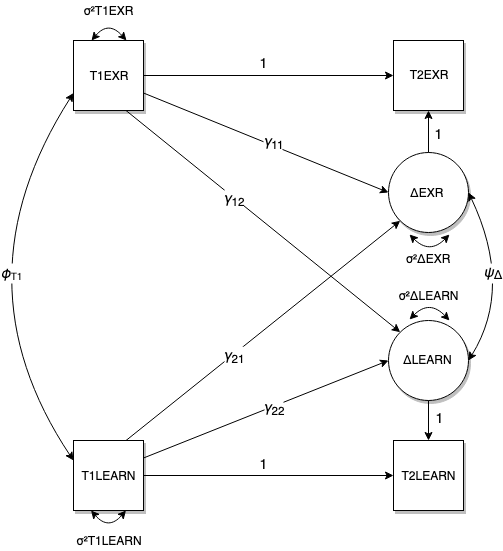
\includegraphics[width=10cm]{Diagram.png}
\caption{Simplified bivariate latent change score model for the effect of exploration and learning at Time 1 on change in exploration and learning from Time 1 to Time 2. Means and item loadings are omitted for visual clarity. Figure adapted from \textcite{Kievit2018}}.
\end{figure}


\begin{figure}[t]
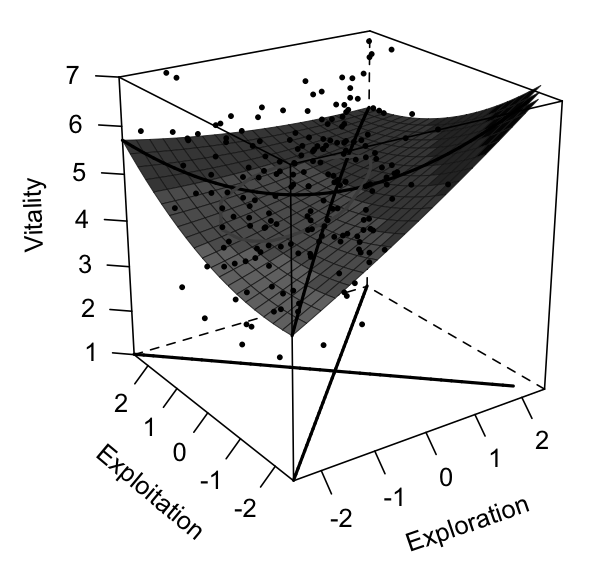
\includegraphics[width=8cm]{Plot.png}
\caption{Response surface plot of the relationships among exploration, exploitation, and vitality at work.}.
\end{figure}

\printbibliography
\end{document}
